\chapter{Fundamentação Teórica}
\label{cap:fundamentacao-teorica}

Neste capítulo, apresenta-se na Seção \ref{sec:levantamento-bibliografico}, o significado do termo Processamento de 
Linguagem Natural (PLN), que é a base para a criação dos algoritmos que se dispõem a fazer a análise e sumarização do texto. Na Seção \ref{sec:normalizacao}, são explicitadas as terminologias utilizadas ao longo dessa pesquisa. Por fim, na Seção \ref{sec:relatedWork}, são discutidos os trabalhos relacionados.

\section{Processamento de Linguagem Natural (PLN)}
\label{sec:levantamento-bibliografico}
O Processamento de Linguagem Natural consiste no desenvolvimento de modelos computacionais para a realização de tarefas que dependem de informações expressas em alguma língua natural (e.g. tradução e interpretação de textos, busca de informações em documentos e interface homem-máquina) \cite{moro2018reconhecimento, do2019processamento}.

De acordo com \citeonline{covington1997prolog}, a pesquisa em PLN está voltada, essencialmente, a três aspectos da comunicação em língua natural:
\begin{itemize}
	\item som: fonologia;
	\item estrutura: morfologia e sintaxe;
	\item significado: semântica e pragmática.
\end{itemize}

A fonologia está relacionada ao conhecimento dos sons que compõem as palavras de uma língua \cite{sousa2022praticas}. A morfologia reconhece as palavras em termos das unidades produtivas que a compõem (e.g. caçou → caç + ou) \cite{lacotizflexao}. A sintaxe define a estrutura de uma frase, com base na forma como as palavras se relacionam nessa frase (Figura \ref{fig:sintaxe}).

\begin{figure}[h]
    \centering
        \caption{Árvore Sintática}
    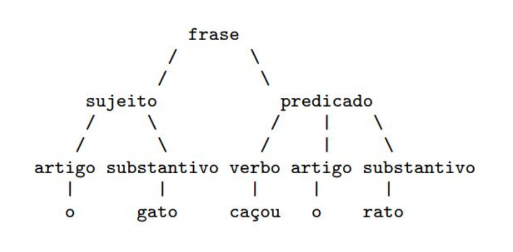
\includegraphics{figuras/figura-1_arvore.png}
    \Fonte{Extraído de \cite{do2019processamento}.} 
    \label{fig:sintaxe}
\end{figure}

A semântica associa significado a uma estrutura sintática, em termos dos significados das palavras que a compõem (e.g. à estrutura da Figura \ref{fig:sintaxe}, podemos associar o significado “um animal 
perseguiu/capturou outro animal”) \cite{de2019unidades}. Finalmente, a pragmática verifica se o significado 
associado à uma estrutura sintática é realmente o significado mais apropriado no contexto considerado (e.g. 
no contexto predador-presa, “perseguiu/capturou” → “comeu”) \cite{moro2018reconhecimento}.

Mesmo com o avanço no relacionamento homem-máquina, a comunicação via linguagem natural continua sendo um 
desafio: como criar programas capazes de interpretar mensagens codificadas em linguagem natural e decifrá-
las para a linguagem de máquina? \cite{silva2021detecccao} Ao longo dos anos, muitas pesquisas e 
desenvolvimentos ocorreram nos mais diversos ramos do processamento de linguagem natural, com ênfase na 
sumarização automática, que a maioria considera ser o ponto de partida para o estudo da linguagem natural 
por meio de computadores \cite{rodriguez2020processamento}.

Para modelar uma linguagem e permitir que as máquinas a compreendam, é necessário um processo de pré-processamento abstrato e estruturado para deixar apenas informações relevantes. Esse pré-processamento reduz o tamanho do vocabulário e torna os dados menos esparsos, um recurso conveniente do processamento computacional \cite{de2020mike}.

A seguir serão descritas as técnicas de processamento da linguagem natural, que são a Normalização (Seção \ref{sec:normalizacao}), Remoção de \textit{Stopwords} (Seção \ref{sec:remocao-stopwords}), Remoção de Numerais (Seção \ref{sec:remocao-numerais}), \textit{Stemização} e Lematização (Seção \ref{sec:stemizacao-lematizacao}), Compreensão da Linguagem Natural (seção \ref{sec:compreensao-linguagem-natural}), e na Seção \ref{sec:terminologia-utilizada} serão descritas as terminologias utilizadas, que são \textit{Tokenização} (Seção \ref{sec:tokenizacao}), Mineração de Textos (Seção \ref{sec:mineracao-textos}) e a Sumarização Automática (Seção \ref{sec:sumarizacao-automatica}).

\subsection{Normalização}
\label{sec:normalizacao}
A normalização abrange tratativas como a \textit{tokenização} \cite{de2022processamento}, transformação de letras 
maiúsculas para minúsculas, remoção de caracteres especiais, remoção de \textit{tags} HTML/Javascript/CSS, 
dentre outras \cite{motta2018estudo}. O processo de \textit{tokenização} visa dividir palavras ou frases em unidades. A \textit{tokenização} lexical \textit{tokeniza} cada palavra como um \textit{token} no texto, reconhecendo-a mesmo que seja tocada por sinais de pontuação \cite{cidrimtecnologias}. 
Um exemplo de texto \textit{tokenizado} lexicalmente seria:
\begin{itemize}
	\item Esta é uma sentença.
	\item[] ['Esta', 'é', 'uma', 'sentença', '.']
\end{itemize} 

A \textit{tokenização} sentencial identifica e marca sentenças. Um exemplo seria:
\begin{itemize}
	\item Esta é a primeira sentença. Esta é a segunda. Esta é a terceira!
	\item[] ['Esta é a primeira sentença.', 'Esta é a segunda.', 'Esta é a terceira!']
\end{itemize}

A normalização é importante por começar a estruturar o texto, já que os processamentos seguintes atuam a partir de unidades sentenciais e lexicais \cite{pinho2021analise}.

\subsection{Remoção de \textit{Stopwords}}
\label{sec:remocao-stopwords}
Uma das tarefas muito utilizadas no pré-processamento de textos é a remoção de \textit{stopwords}. Esse 
método consiste em remover palavras muito frequentes, tais como “a”, “de”, “o”, “da”, “que”, “e”, “do” 
entre outras, pois na maioria das vezes não são informações relevantes para a construção do modelo 
\cite{dos2021analise}. 
Esse processo, só pode ser aplicado quando realmente as palavras não forem importantes para a compreensão do 
sentido do texto.

\subsection{Remoção de Numerais}
\label{sec:remocao-numerais}
Outra remoção necessária é a dos numerais presentes no texto. Os numerais não agregam informação relevante 
por não trazerem carga semântica \cite{jurafskymartin2020}. O PLN remove também os símbolos que os 
acompanham, como “R\$”, “\$”, “US\$”, “km”, “milhões”, “bilhões”, dentre outros.

\subsection{Stemização e Lematização}
\label{sec:stemizacao-lematizacao}
O processo de \textit{stemização} (do inglês, \textit{stemming}) consiste em reduzir uma palavra ao seu 
radical \cite{gobbo2019abordagem}. A palavra “meninas” se reduziria a “menin”, assim como “meninos” e 
“menininhos”. As palavras “gato”, “gata”, “gatos” e “gatas” reduzem-se para “gat”. A lematização reduz a 
palavra ao seu lema, que é a forma no masculino e singular. No caso de verbos, o lema é o infinitivo 
\cite{campos2021uso}.

Por exemplo, as palavras “gato”, “gata”, “gatos” e “gatas” são todas formas do mesmo lema: “gato”. 
Igualmente, as palavras “tiver”, “tenho”, “tinha”, “tem” são formas do mesmo lema “ter”. A vantagem de 
aplicar a \textit{stemização} ou lematização é clara: redução de vocabulário e abstração de significado
\cite{santos2022processamento}.

\subsection{Compreensão da Linguagem Natural}
\label{sec:compreensao-linguagem-natural}
Essa parte do processamento de linguagem natural é responsável por transformar sentenças de um texto em 
estruturas lógicas, ou seja, é compreender uma frase que carrega um valor que pode ser verdadeiro ou falso 
\cite{frutuoso2018processamento}.

A compreensão da linguagem natural tem como objetivo facilitar a manipulação de texto por computadores, além 
de identificar instruções recebidas por humanos e até por outras máquinas. É o processo de construção de uma 
base semântica formal da linguagem. O significado atribuído a sentenças pode ser interpretado pelo 
computador, da mesma forma que os humanos o fazem \cite{d2022inteligencia}.

\section{Terminologia Utilizada}
\label{sec:terminologia-utilizada}
Esta seção, apresenta as principais terminologias utilizadas no decorrer dessa pesquisa.

\subsection{Tokenização}
\label{sec:tokenizacao}
Uma das principais etapas da operação de normalização é a \textit{tokenização}, que é realizada com o objetivo de quebrar um documento de texto nas menores unidades, mas que representem a mesma semântica original do texto. É usado durante o processamento de linguagem natural para segmentação de palavras, localizando caracteres para quebrar sequências de caracteres no texto Limites por palavra, ou seja, palavras separadas ou frases em unidades \cite{rodriguez2020processamento}.

A \textit{tokenização} também foi exemplificada na Seção \ref{sec:normalizacao}.

\subsection{Mineração de Textos}
\label{sec:mineracao-textos}
A mineração de textos é um conjunto de métodos utilizado para navegar, organizar, encontrar e descobrir informações em bases textuais \cite{deuso}.

A tecnologia de mineração de textos deriva das técnicas de recuperação de informações e da descoberta de informações estruturadas, por meio do uso de bancos de dados e de procedimentos estatísticos \cite{lima2022big}. É uma subárea da extração de informações, porém é utilizada somente para análise em textos.

Por mais que possa parecer similar, a mineração de textos é diferente de mecanismos de busca, uma vez que 
na busca o usuário já sabe o que quer encontrar; enquanto na mineração de textos, o usuário descobrirá conhecimento e padrões até então, por ele desconhecidos \cite{souza2021modelo}. Em suma, na busca o usuário pesquisa determinada informação e na mineração é realizada a coleta de novos conhecimentos “escondidos” nos textos.

Mineração de textos \cite{ferreira2021mineraccao} é o processo de extrair conhecimento não conhecido previamente a partir de fontes textuais, tais como correio, imprensa, transações, \textit{websites}, \textit{newsgroups}, fóruns, listas de correspondência, redes sociais, dentre outros.

\subsection{Sumarização Automática}
\label{sec:sumarizacao-automatica}
A sumarização automática é o processo de selecionar as informações mais importantes de um conjunto de
fontes, seja um único texto ou um corpus, para produzir uma versão resumida \cite{martins2001introduccao}.

Os textos podem ser de qualquer tipo: notícias, artigos científicos, postagens em blogs, resenhas de filmes, atas de reuniões e muito mais. Eles também podem ser escritos em qualquer idioma sem a necessidade de uma escrita formal ou casta. Obviamente, os métodos de resumo, incluindo algum pré-processamento, podem variar de idioma para idioma, com a grande maioria existente para o inglês \cite{cabral2014platform}.

Computacionalmente explicando, existem duas formas de se abordar o problema da sumarização, a superficial e
a profunda \cite{salvino2019analise}. Neste trabalho será abordada a primeira, que utiliza métodos 
estatísticos e/ou empíricos para obter o sumário. Essa técnica é a mais simples de ser implementada e é 
utilizada por grande parte dos pesquisadores, porém, pode produzir sumários com problemas de coesão e 
principalmente de coerência, o que pode deixar o resumo sem um sentido lógico da ordem das frases, 
apresentando deficiências no sentido das frases \cite{antunes2018abordagem}. Por outro lado, a sumarização profunda realiza uma análise semântica frase a frase no texto, analisando a forma que as frases são 
construídas e o relacionamento de uma frase a outra \cite{pinho2021analise}.

\section{Trabalhos Relacionados}
\label{sec:relatedWork}
Esta seção, visa apresentar alguns trabalhos relacionados ao Processamento de Linguagem Natural.
%
Em \citeonline{singh2018natural}, são apresentadas as sub-tarefas da tecnologia de extração de informações, 
além de destacar pesquisas de ponta em várias tarefas onde a extração de informação é utilizada. Além disso, 
o artigo destaca os desafios atuais de lidar com o Processamento de Linguagem Natural, em razão da explosão 
de informações na forma de notícias, artigos, redes sociais, mídia, de uma forma que todo o texto 
interpretado pela máquina consiga ser identificado, extraído e repassado para o usuário de uma forma 
entendível.

\citeonline{rodriguez2020processamento} apresentam uma forma alternativa de integração do meio jurídico com a 
tecnologia, expondo meios de como o Processamento de Linguagem Natural poderia ajudar a automatizar o 
reconhecimento de Entidades Nomeadas (Agentes Públicos) em uma base de portaria. Eles utilizam o NLTK 
(\textit{Natural Language Toolkit}), que junto da linguagem de programação \textit{Python}, trabalham com 
dados de linguagem humana para aplicação do PNL. O NLTK é útil para separar as sentenças em um paragrafo, 
separar as palavras dentro de cada sentença, reconhecer padrões no texto e criar modelos de classificação que 
permitam identificar nomes próprios dentro de um conjunto de dados.

\citeonline{vieira2019analise} apresentam uma análise descritiva acerca do conteúdo das notícias publicadas 
no Portal da Saúde, através da utilização da técnica de mineração de textos, onde tentam gerar insumos e 
informações para discussões sobre o impacto da \textit{fake news} na área da saúde. A ideia vem da análise de 
uma iniciativa lançada pelo Ministério da Saúde sobre o enfrentamento de notícias falsas que tem se espalhado 
nas mais diversas áreas, como política, finanças e a própria saúde, que se chama "Saúde sem 
\textit{fake news}".

\citeonline{tabosa2020avaliaccao} apresenta uma pesquisa iniciada no ano de 2014 sobre o desenvolvimento de 
um \textit{software} que fosse capaz de criar resumos automáticos de textos baseados em técnicas de PLN, 
baseando-se na frequência de palavras. Os primeiros testes dessa ferramenta geraram resultados que indicavam 
uma significativa redução da dimensionalidade dos textos, preservando seu valor semântico. O artigo apresenta 
os resultados dessa pesquisa mostrando que existiu uma equivalência qualitativa entre os resumos produzidos 
pela ferramenta e por humanos, mas que deixa a desejar quando se trata do tamanho do resumo gerado, visto que 
o resultado da sumarização feita pela ferramenta denota textos muito longos.

O algoritmo de Marques apresentado neste trabalho foi comparado com outros algoritmos de sumarização automática de texto presentes na literatura. Dentre os trabalhos relacionados, destacam-se os algoritmos GistSumm, Luhn, PLI, Regressão Bayesiana e ChatGPT. A Tabela  \ref{tab:comparacao_marques_trabalhos_relacionados} apresenta as principais diferenças entre o algoritmo de Marques e os algoritmos relacionados.

O algoritmo de Marques se destaca em relação aos algoritmos relacionados por utilizar um modelo de redes neurais treinado especificamente para a tarefa de sumarização automática de textos.

\begin{table}[ht]
\centering
\caption{Comparação entre o algoritmo de Marques e algoritmos relacionados}
\label{tab:comparacao_marques_trabalhos_relacionados}
    \begin{tabular}{|l|p{6cm}|p{6cm}|}
    \hline
        \textbf{Algoritmo} & \textbf{Características} & \textbf{Diferenciais em relação ao algoritmo de Marques} \\ \hline
        GistSumm & Baseado em técnicas de extração & Menor desempenho em precisão, coerência e coesão \\ \hline
        Luhn & Utiliza frequência de palavras e posição no texto & Inferior em termos de precisão e coerência \\ \hline
        PLI & Baseado em programação linear inteira & Desempenho inferior nas métricas de qualidade \\ \hline
        Regressão Bayesiana & Abordagem baseada em aprendizado de máquina & Tempo de processamento mais lento \\ \hline
        ChatGPT & Geração de resumos por modelo pré-treinado de linguagem & Tempo de processamento mais lento e desempenho inferior nas métricas de qualidade \\ \hline
        Marques & Redes neurais treinadas especificamente para sumarização automática de textos & Melhor desempenho em precisão, coerência, coesão e tempo de processamento \\ \hline
    \end{tabular}
\end{table}